% !TEX root = ../thesis.tex
\chapter{Introduction} \label{cha:intro}
\section{Task}
\section{Background}
% This thesis covers the development and engineering process of the \gls{EDiC} pictured in \cref{fig:EDiCSnake}.
% It is a completely novel \gls{CPU} architecture built to visualize and show the fundamental workings of any \gls{CPU}.
% The \gls{EDiC} can execute over half a million instructions per second but also features step-by-step, instruction-by-instruction as well as breakpoint capabilities for better understanding of how \glspl{CPU} work.
% All components can be tested individually with the help of dedicated test adapters and, therefore, \gls{IC} failures can be tracked down and fixed easily.
% Additionally to the hardware built, the project includes an open source development environment including an assembler, tools to modify the micro-code and also \gls{FPGA} simulation and emulation of the hardware \cite{EDiCGitHub}.
% \begin{figure}[t]
%   \centering
%   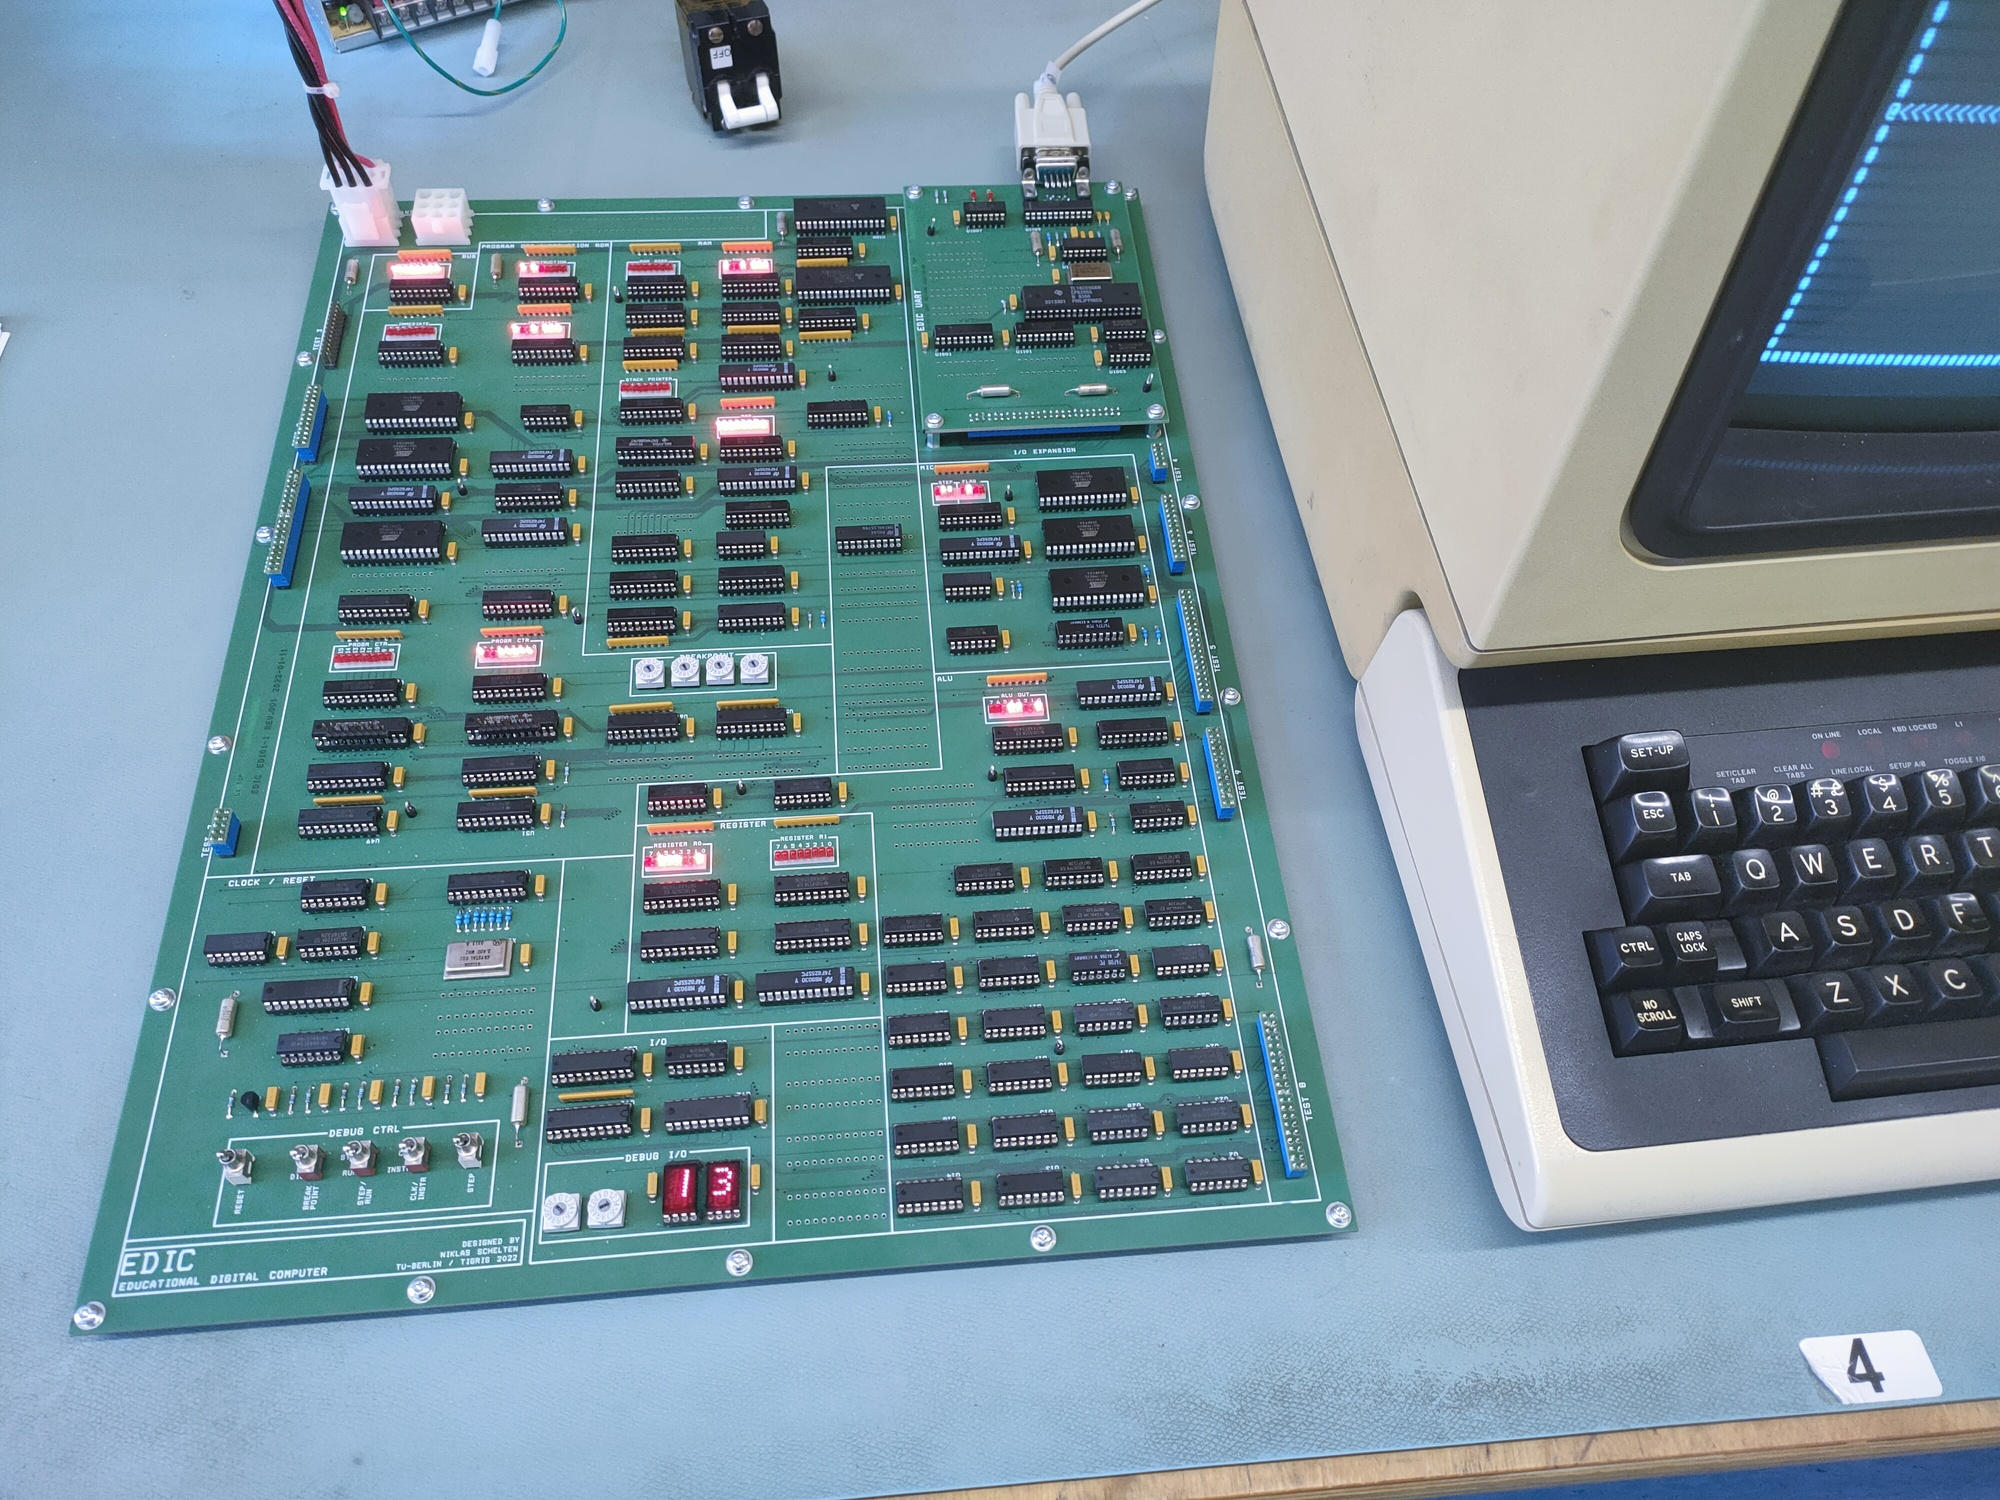
\includegraphics[width=\textwidth]{IMG20220308163628_resize.jpg}
%   \caption{The final version of the \gls{EDiC} playing Snake on a VT-100 over an RS-232 I/O card.}
%   \label{fig:EDiCSnake}
% \end{figure}

% \section{The Beginning}
% The foundation of this project started at the end of 2020 where I decided to design and build a \gls{CPU} from scratch.
% In many university courses we would discuss some parts of a \gls{CPU} like different approaches to binary adders or pipelining concepts but never would we build a complete \gls{CPU} including the control logic.
% Due to a Covid-19 lockdown I had enough time at my hands and after 6 years of study, I felt like I had the expertise to complete this project.

% \begin{figure}[t]
%   \centering
%   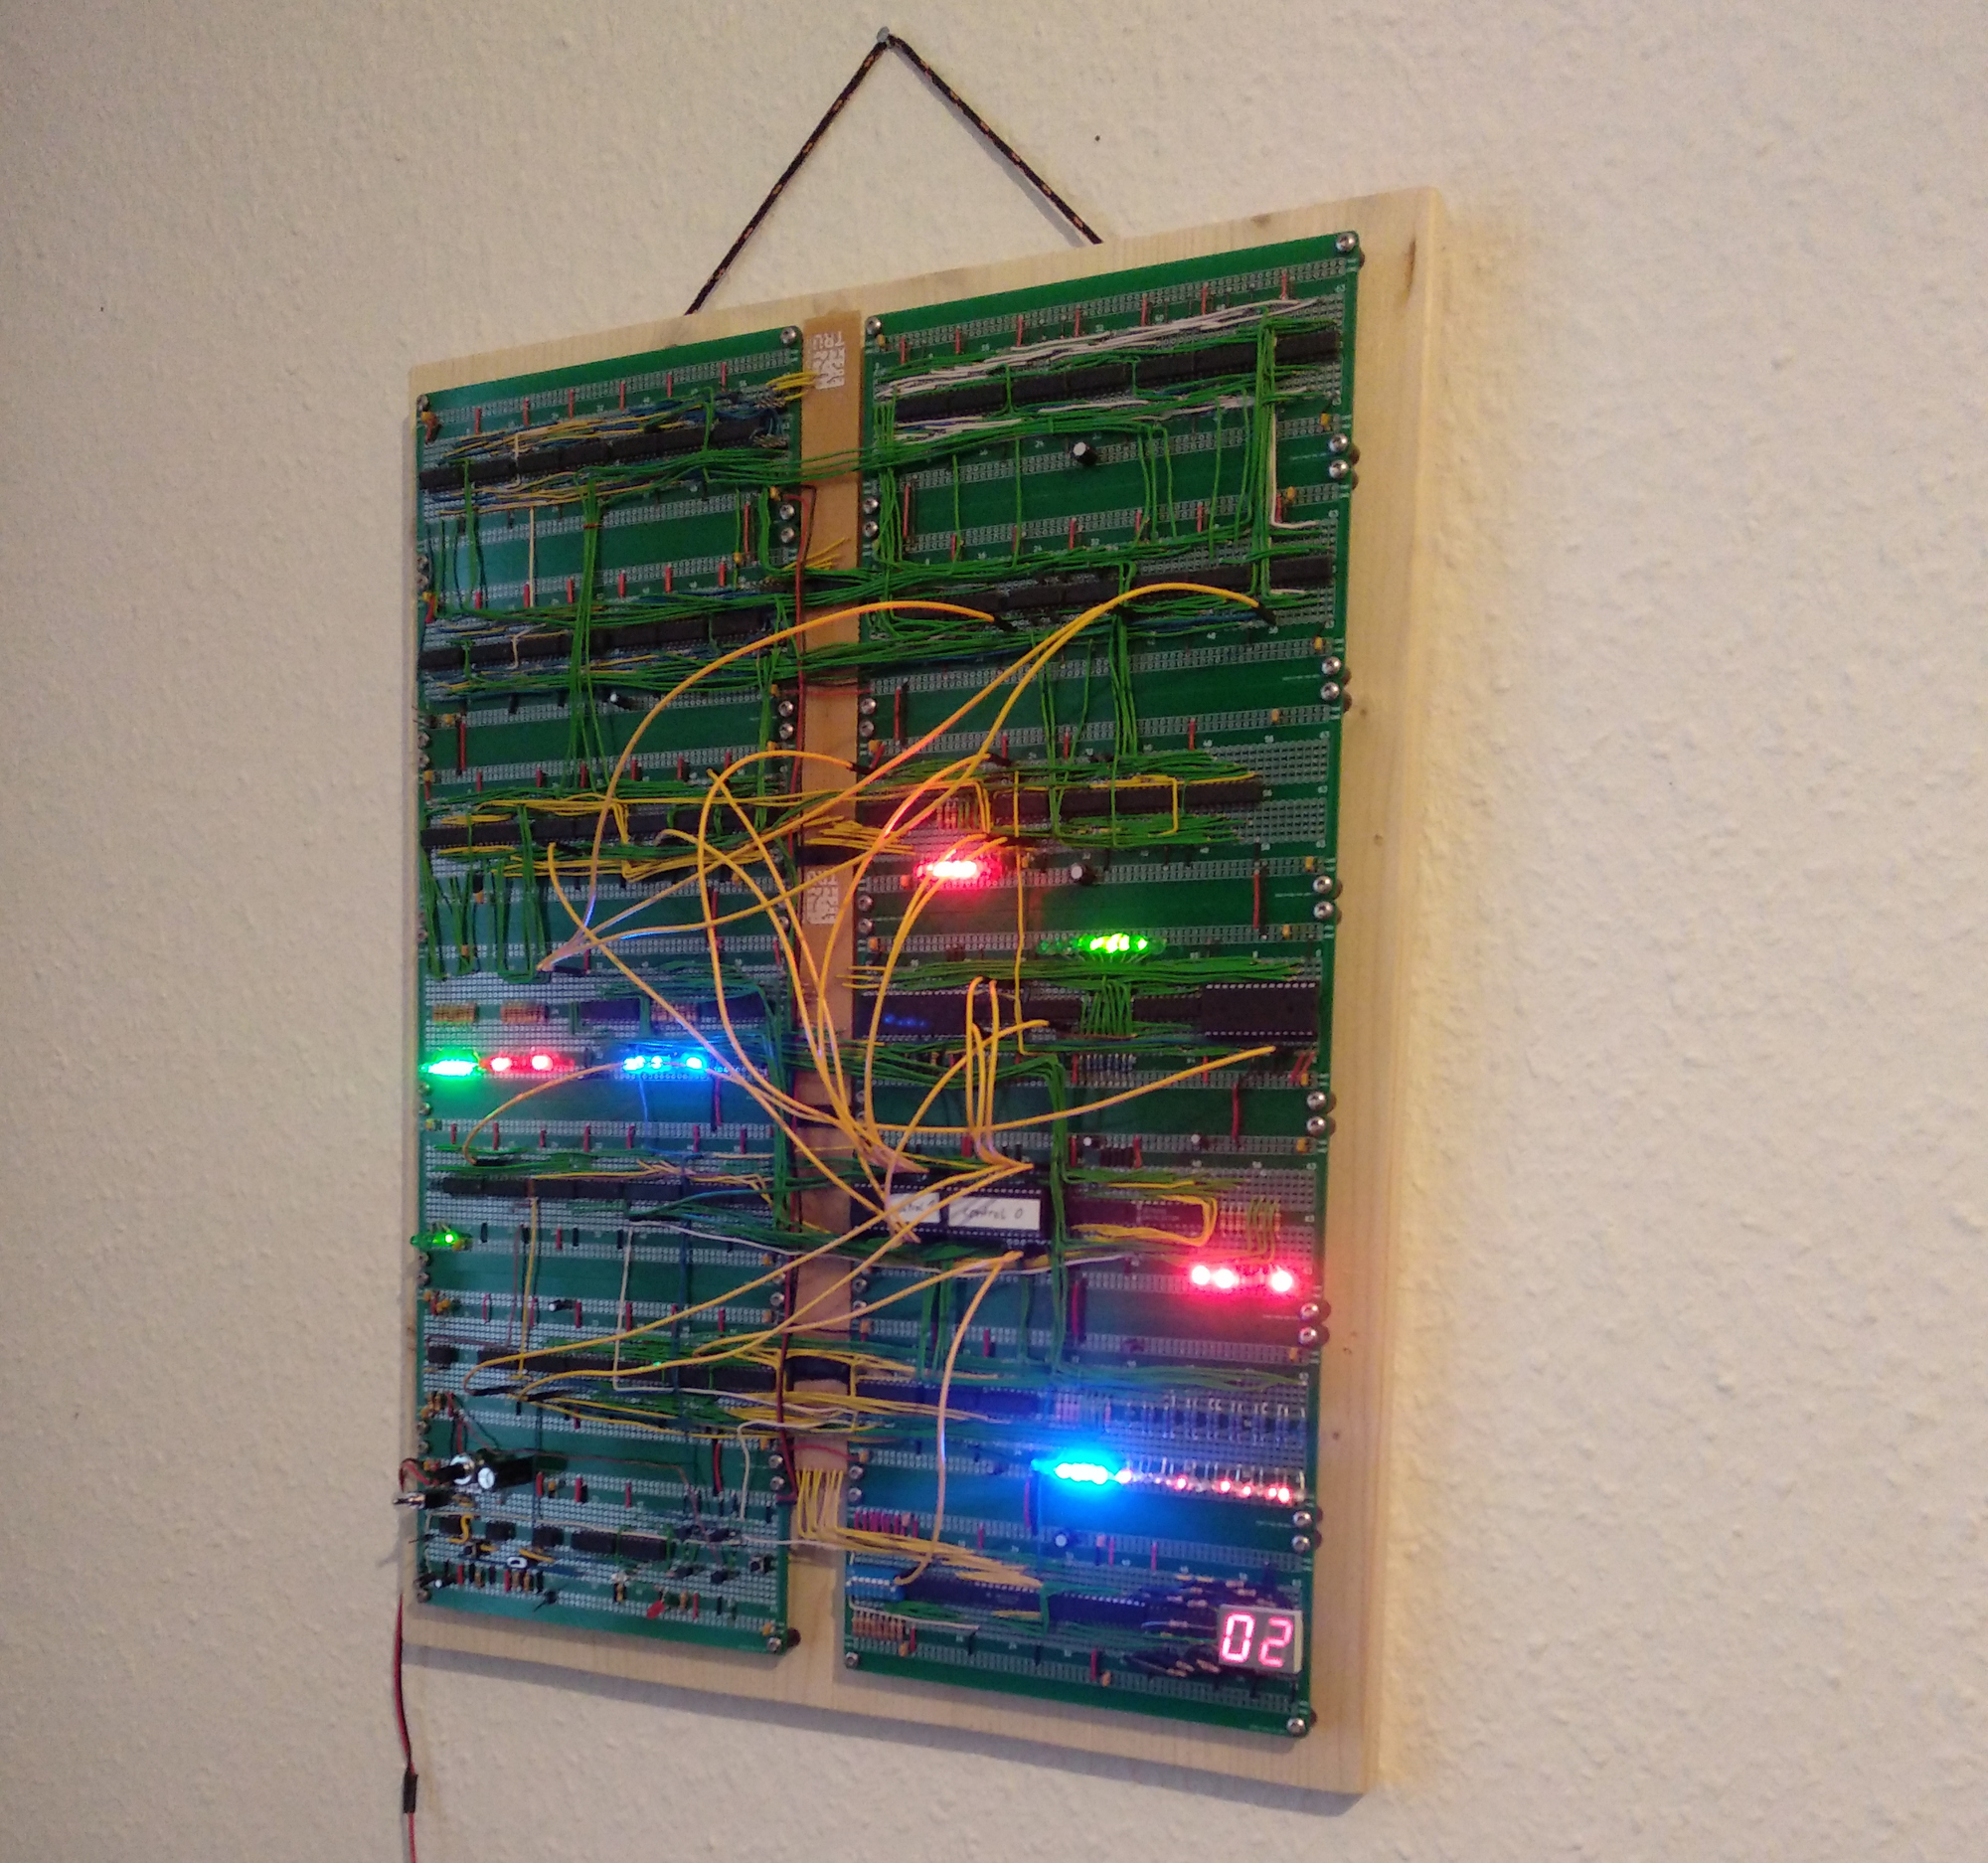
\includegraphics[width=\textwidth]{update20210121_crop_res.jpg}
%   \caption{The first version of the \gls{CPU} in its final state.}
%   \label{fig:initialCPU}
% \end{figure}
% At the end of January 2021 I succeeded with the actual hardware built and the \gls{CPU} was able to execute a prime factorization of 7 bit numbers.
% \Cref{fig:initialCPU} depicts the final hardware build.
% Its design ideas, implementation and flaws are shown in \cref{cha:prev}.
% \TODO{rewrite to current chapters}

% Through the university module ``Mixed-Signal-Baugruppen'' I got to know Henry Westphal in summer 2021.
% He established a company that builds mixed-signal-electronics and, therefore, has a deep understanding of analog and digital circuitry.
% As he heard of my plans to build a future version of my \gls{CPU} he was immediately interested and we wanted to rebuild a \gls{CPU} with some changes:
% \begin{itemize}
%   \item The general architecture should remain similar to the existing \gls{CPU} with only changes where it was necessary.
%   \item The objective was no longer only to create a functioning \gls{CPU}, this was already accomplished, but the build should be such that it could be used for education.
%   \item It should be more reliable, more capable and its components should be easily distinguishable. Therefore, it is to be build on a large \gls{PCB}.
%   \item There should be a generic interface for extension cards, i.e. IO Devices.
% \end{itemize}
% How the, now called, \gls{EDiC} differs from its predecessor is presented in \cref{cha:architecture}.

% To achieve the goal of the \gls{EDiC} being educational it is important to not only build the hardware but to also provide a Software Environment to, for example, write applications.
% This is presented in \cref{cha:software}.

% An important step in the design of the \gls{EDiC} was to thoroughly simulate and implement the behavior on an \gls{FPGA}.
% I firstly simulated the behavior and after the hardware schematic was finished, we built a script to convert the exported netlist to verilog to simulate the \gls{CPU} on chip level.
% The process and differences between the \gls{FPGA} design and the actual hardware are presented in \cref{cha:fpga}.

% \Cref{cha:hardware} describes the final hardware assembly, commissioning and timing analysis to determine the final clock frequency.

% The final conclusion and future improvements are given in \cref{cha:conclusion}.


% \label{sec:outputBuffer}
% \TODO{Explain output buffer and why low level outputs have higher current ratings}